\documentclass[fleqn]{scrartcl}
\usepackage[T1]{fontenc}
\usepackage[utf8x]{inputenc}
\usepackage[ngerman]{babel}
\usepackage{scrpage2}
\usepackage{paralist}
\usepackage{titling}
\usepackage{tabularx}
\usepackage{amsmath}
\usepackage{amsfonts}
\usepackage{amssymb}
\usepackage{mathtools}
\usepackage{ucs}
\usepackage[shortlabels]{enumitem}
\usepackage{graphicx}
\usepackage{listings}
\usepackage{tikz}
\usepackage{xcolor}

\definecolor{deepblue}{rgb}{0,0,0.5}
\definecolor{deepred}{rgb}{0.6,0,0}
\definecolor{deepgreen}{rgb}{0,0.5,0}

\lstset{
language=Python,
breaklines=true,
otherkeywords={self,nonlocal},             % Add keywords here
keywordstyle=\bfseries\color{orange},
emph={__init__},          % Custom highlighting
emphstyle=\color{deepred},    % Custom highlighting style
stringstyle=\color{deepgreen},
frame=tb,                         % Any extra options here
showstringspaces=false,            % 
numbers = left
}

\pagestyle{scrheadings}
\clearscrheadfoot
\cfoot[\pagemark]{\pagemark}
\author{Tom Schmidt\\ \and Stefan Poggenberg\\ \and Samuel Schöpa\\216203821 \and Bjarne Hiller\\216203851}
\title{KI HA 1}
\date{18. Mai 2018}

\begin{document}
\maketitle
\section{Der Staubsauger-Agent}
\subsection{Implementierung}
\lstinputlisting[firstline=87, lastline=121]{a1/a1.py}
\subsection{Optimaler Agent}
Der implementierte Agent ist nicht optimal, da er für die Auswahl seiner Aktion nur die momentan benachbarten Felder beachtet. Sind alle benachbarten Felder schon entdeckt, wählt er eine zufällige Aktion. Ein optimaler Agent würde stattdessen berücksichtigen, in welche Richtung er sich bewegen müsste, um am schnellsten zu unbekannten Feldern zu kommen. Dies wäre dann aber schon ein Ziel-basierter Agent, da er zukünftige Beobachtungen und Aktionen berücksichtigt. Außerdem dürfte ein optimaler Agent keine Bewegungen mehr ausführen, wenn er sich sicher ist, dass er die gesamte Umgebung erkundet hat und alles sauber ist, da er so Performance verliert. Dies ist aber in der gegebenen Multi-Agent-Umgebung schwierig zu implementieren, da Felder nicht nur vom statischen Rand, sondern auch von anderen mobilen Agenten blockiert werden können.
\section{Problemlösen durch Suchen}
\subsection{Suchalgorithmen}
\begin{enumerate}[a)]
\item
\begin{enumerate}[i.]
\item Breitensuche: $[\text{Start},7,\text{Ziel}]$\\
\begin{tabularx}{\linewidth}{|l|X|}
\hline
Node&Queue\\
\hline\hline
Start&1, 2, 7\\\hline
1&2, 7, 4\\\hline
2&7, 4, 5, 6\\\hline
7&4, 5, 6, Ziel\\\hline
4&5, 6, Ziel, 8\\\hline
5&6, Ziel, 8\\\hline
6&Ziel, 8, 3\\\hline
Ziel&8\\\hline
\end{tabularx}
\item Tiefensuche: $[\text{Start},1,4,8,\text{Ziel}]$\\
\begin{tabularx}{\linewidth}{|l|X|}
\hline
Node&Stack\\
\hline\hline
Start&7, 2, 1\\\hline
1&7, 2, 4\\\hline
4&7, 2, 8\\\hline
8&7, 2, Ziel\\\hline
Ziel&7, 2, 6\\\hline
\end{tabularx}
\item A*: $[\text{Start},2,6,\text{Ziel}]$\\
\begin{tabularx}{\linewidth}{|l|X|}
\hline
Node&Discovered\\
\hline\hline
Start&\textcolor{blue}{1 ($85+272=357$)}, 2 ($217+219=436$), 7 ($173+383=556$)\\\hline
1&2 ($436$), 7 ($556$), \textcolor{blue}{4 ($85+80+253=418$)}\\\hline
4&\textcolor{blue}{2 ($436$)}, 7 ($556$), 8 ($85+80+250+57=472$)\\\hline
2&7 ($556$), 8 ($472$), 5 ($217+186+318=721$), \textcolor{blue}{6 ($217+103+150=470$)}\\\hline
6&7 ($556$), \textcolor{blue}{8 ($472$)}, 5 ($721$), 3 ($217+103+183+189=692$), Ziel ($217+103+167=487$)\\\hline
8&7 ($556$), 5 ($721$), 3 ($692$), \textcolor{blue}{Ziel ($85+80+250+84=499 > 487$)}\\\hline
\textcolor{blue}{Ziel (487)}&7 ($556$), 5 ($721$), 3 ($692$)\\\hline
\end{tabularx}
\item Greedy: $[\text{Start},2,6,\text{Ziel}]$\\
\begin{tabularx}{\linewidth}{|l|X|}
\hline
Node&Discovered\\
\hline\hline
Start&1 ($272$), \textcolor{blue}{2 ($219$)}, 7 ($383$)\\\hline
2&1 ($272$), 7 ($383$), 5 ($318$), \textcolor{blue}{6 ($150$)}\\\hline
6&1 ($272$), 7 ($383$), 5 ($318$), \textcolor{blue}{Ziel (0)}\\\hline
\textcolor{blue}{Ziel}&1 ($272$), 7 ($383$), 5 ($318$)\\\hline
\end{tabularx}
\end{enumerate}
\item
\begin{enumerate}[i.]
\item Breitensuche\\
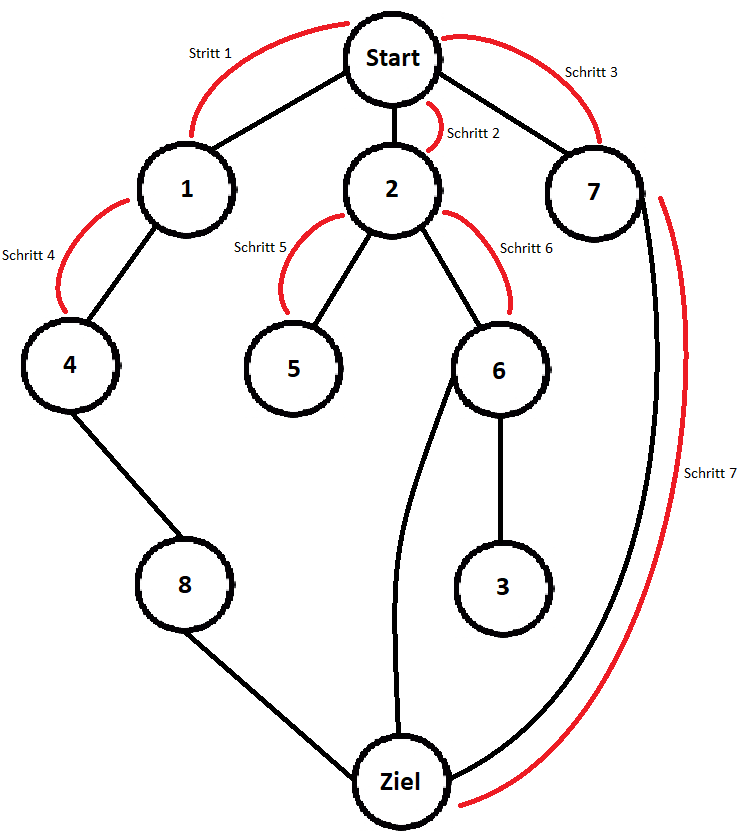
\includegraphics[width=\linewidth]{pictures/breadth-first-search.png}
\item Tiefensuche\\
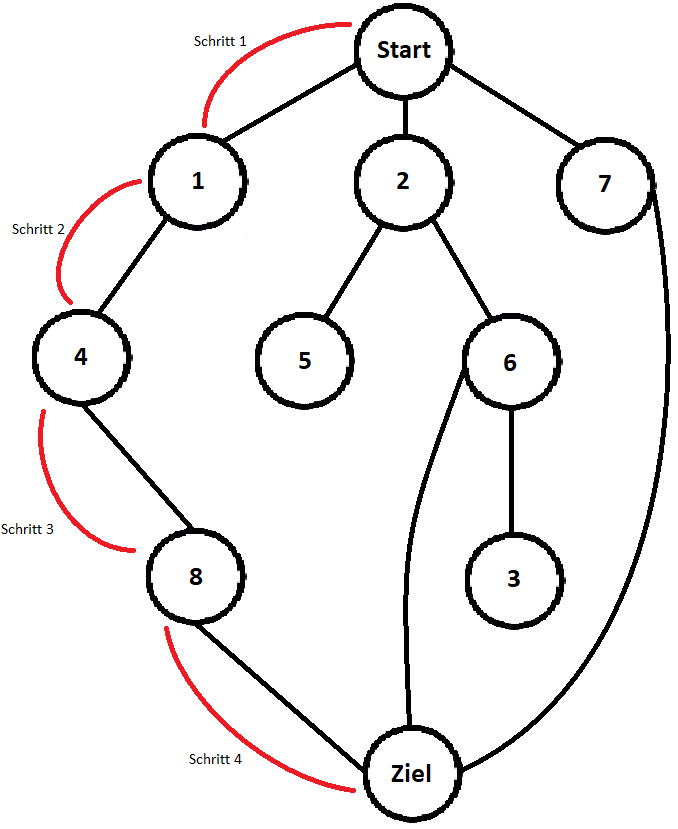
\includegraphics[width=\linewidth]{pictures/depth-first-search.png}
\item A*\\
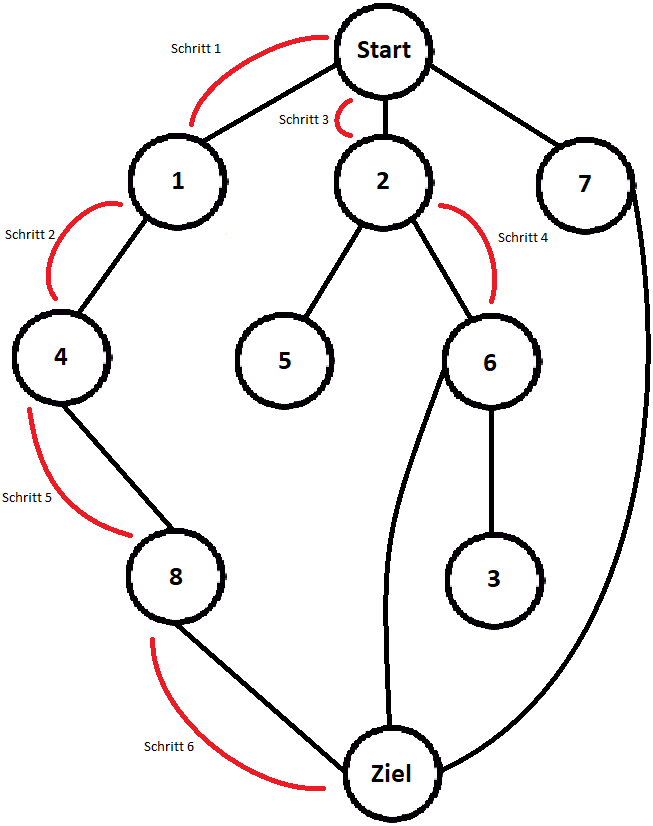
\includegraphics[width=\linewidth]{pictures/a-star-search.png}
\item Greedy\\
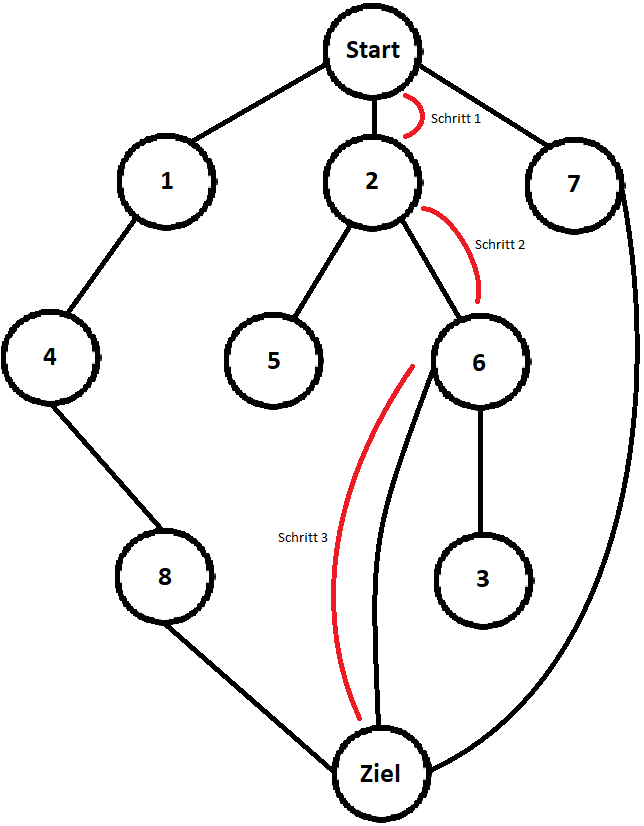
\includegraphics[width=\linewidth]{pictures/greedy-search.png}
\end{enumerate}
\end{enumerate}

\subsection{Implementierung}
\lstinputlisting[firstline=151, lastline=164,title=(a) Definition des Graphen]{a2/a2.py}
\lstinputlisting[firstline=63, lastline=80,title=(b) Heuristik]{a2/a2.py}
\lstinputlisting[firstline=113, lastline=139,title=(c) Greedy-Suche]{a2/a2.py}
\lstinputlisting[firstline=168,title=(d) main-Funktion]{a2/a2.py}
\end{document}
